%%%%%%%%%%%%%%%%%%%%%%%%%%%%%%%%%%%%%%%%%%%%%%%%%%%%%%%%%%%%%%%%%%%%%%%%%%%%%%%%


%\documentclass[letterpaper, 10pt, conference]{IEEEtran}
\documentclass[notes]{beamer}
\usepackage{tikz}
\usetikzlibrary{calc,decorations.markings,arrows, fadings}
\usepackage{tikz-timing}
\usepackage{media9}
%\usepackage{multimedia}
\usepackage{amsmath}
\usepackage{xifthen}
\usepackage{amsfonts}
\usepackage{tabu}
\usepackage{graphicx,dblfloatfix}
\usepackage[font=small]{caption}
%\usepackage{subcaption}
\usepackage{cite}
\usepackage{placeins}
\usepackage{xspace}
\usepackage{subfiles}
\usepackage{url}
\usepackage[outline]{contour}
\usepackage{hyperref}
\contourlength{0.18em}

\usetheme{Copenhagen}
\usecolortheme{beetle} 
%\setbeamertemplate{navigation symbols}{}
\beamertemplatenavigationsymbolsempty
\setbeamerfont{footline}{series=\scriptsize}
\usefonttheme{structurebold}

\definecolor{beetle@other}{RGB}{207,184,124} %cu gold
%
%Once I break this in to multiple sections, each section will be added with:
%	\subfile{filename}
%In those other files, I have as preamble:
%	\documentclass[main.tex]{subfiles}
%

\title[\textcolor{black}{Low-Cost Omnidirectional Powertrain}]{A Stick-Slip Omnidirectional Powertrain for Low-Cost Swarm Robotics:\\ Mechanism, Calibration, and Control}
\author[{\tt john.klingner@colorado.edu}]{John Klingner, Anshul Kanakia, Nicholas Farrow, Dustin Reishus and Nikolaus Correll}
\institute[]{Department of Computer Science\\University of Colorado Boulder}
\date{}

\newcommand{\Tau}{\boldsymbol{\mathrm{T}}}

\begin{document}
\begin{frame}
	\titlepage
\end{frame}
\begin{frame}{Motivation \& Background}
\begin{columns}[c]
	\column{0.65\textwidth}
		\begin{itemize}
			\item Stick-slip motion.
			\begin{itemize}
				\item Think of the way a vibrating cell phone moves across a tabletop.
				\item Low cost, compact, and simple.
			\end{itemize}
				\note[item]<1->{
					\begin{itemize}
						\item "Stick-slip" motion uses the forces of a vibration motor to cause the robot platform to scoot across the ground. The figure on the bottom shows a simplified, single degree-of-freedom example in which the vibration motor is shown as a rotating mass.
						\item Main motivation behind this is that the actuators are low in cost and complexity and small in size.
						\item We extend this to use three motors, allowing the platform to move in any direction, but previous work has only demonstrated this principle in hardware with two motors.
						\item This lower cost and simplicity is particularly helpful when fielding large swarms of robots.
						\item We implemented and tested this design on the Droplets swarm robotics platform.
					\end{itemize}
				}
		\end{itemize}
	\column{0.35\textwidth}
		\begin{figure}
			\centering
			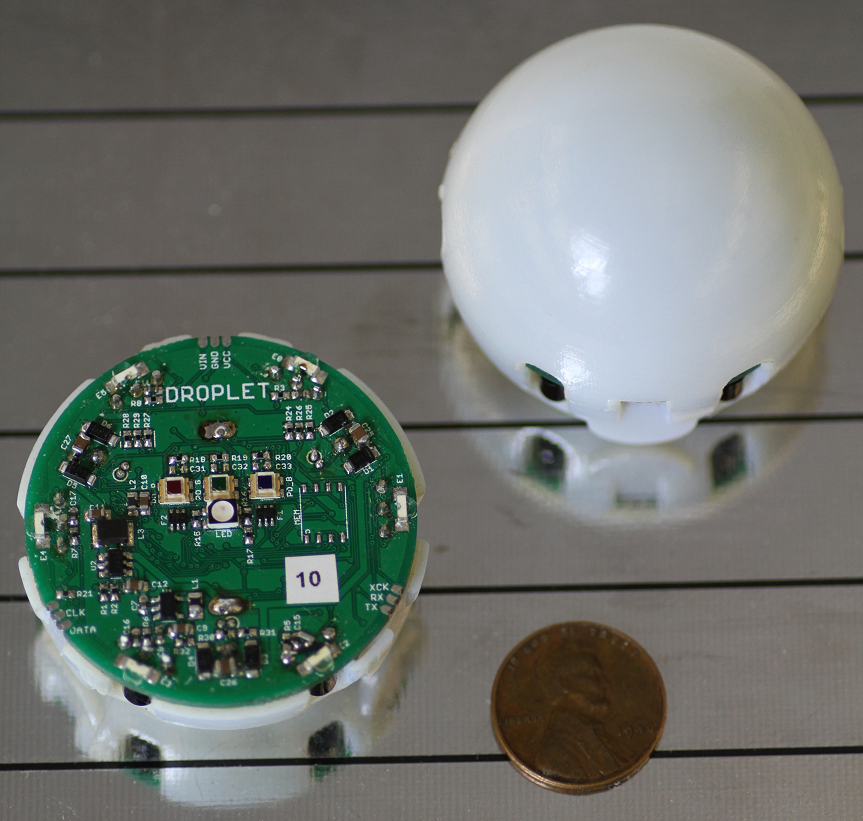
\includegraphics[width=\textwidth]{Images/droplets.png}
		\end{figure}
\end{columns}
		\begin{figure}
			\centering
			\makebox[\textwidth][c]{
			\subfile{singleDoFModelPresentation}
			}
		\end{figure}
\end{frame}
\begin{frame}
	\begin{figure}
		\centering
				\includemedia[activate=pagevisible, noplaybutton, width=\textwidth,flashvars={loop=true}]{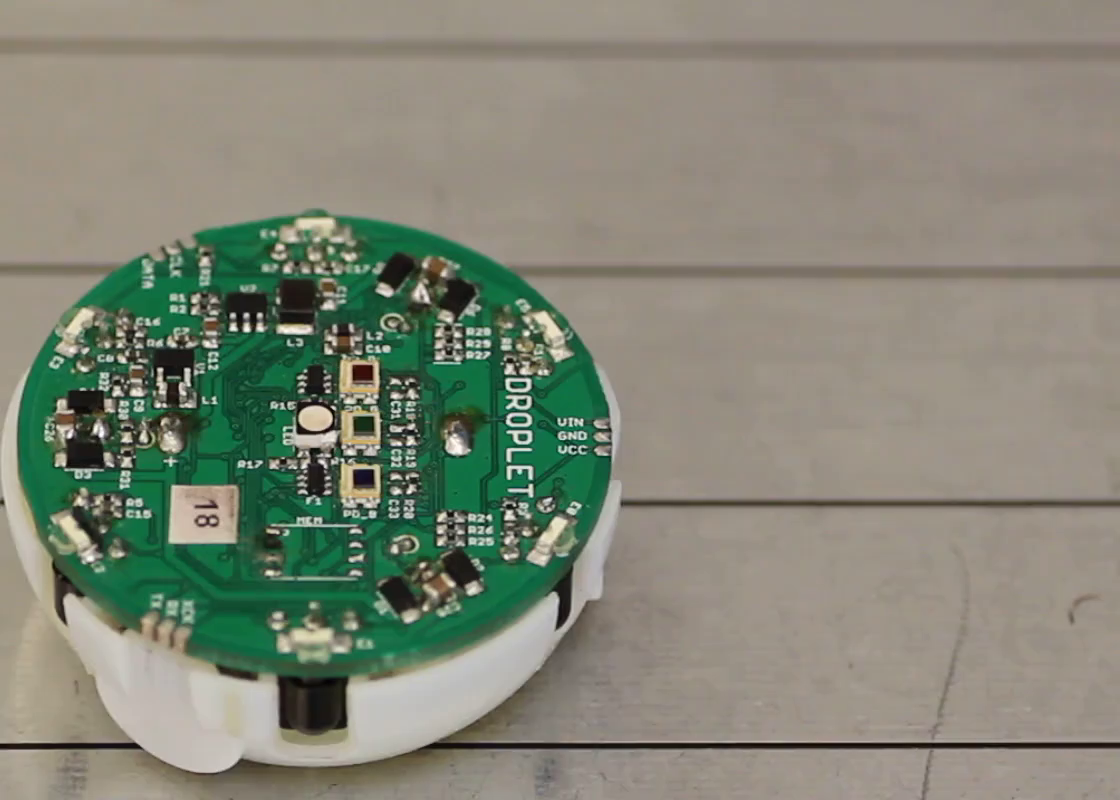
\includegraphics{Images/realWalking.png}}{Images/realWalking.swf}
	\end{figure}
	\note{We implemented and tested this design on the Droplets swarm robotics platform, and I have a few robots to demonstrate with in the poster session.}
\end{frame}
\begin{frame}
	\frametitle{Mechanism}
	\begin{columns}[c]
		\column{0.6\textwidth}
			\begin{itemize}
				\item Motors opposite legs.
					\note[item]<1->{With motors positioned opposite the robots' legs, the motor's rotation causes the robot to pivot about the opposite leg.}
				\item One motor on at a time gives `steps'.
					\note[item]<1->{One motor is turned on for a brief time, causing the robot to take a small step.}
				\item Chain together a sequence of steps to walk.
					\note[item]<1->{To walk, the robot chains together a sequence of these steps.}
			\end{itemize}
		\column{0.4\textwidth}
			\begin{figure}
				\centering
				\includemedia[activate=pagevisible, noplaybutton, width=\textwidth,flashvars={loop=true}]{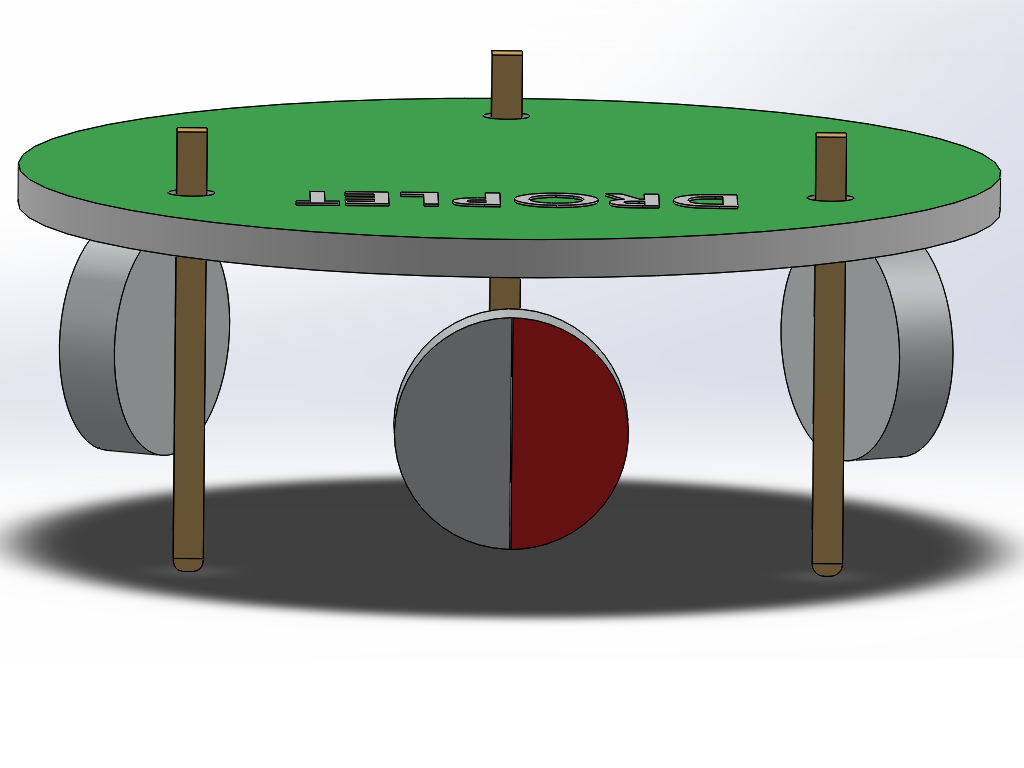
\includegraphics{Images/Step.png}}{Images/Step.swf}
			\end{figure}
			\note[item]<1->{This animation is an exaggerated demonstration of a single `step'. In practice one step takes about $30$ms.}
			\begin{figure}
				\centering
				\includemedia[activate=pagevisible, noplaybutton, width=0.8\textwidth]{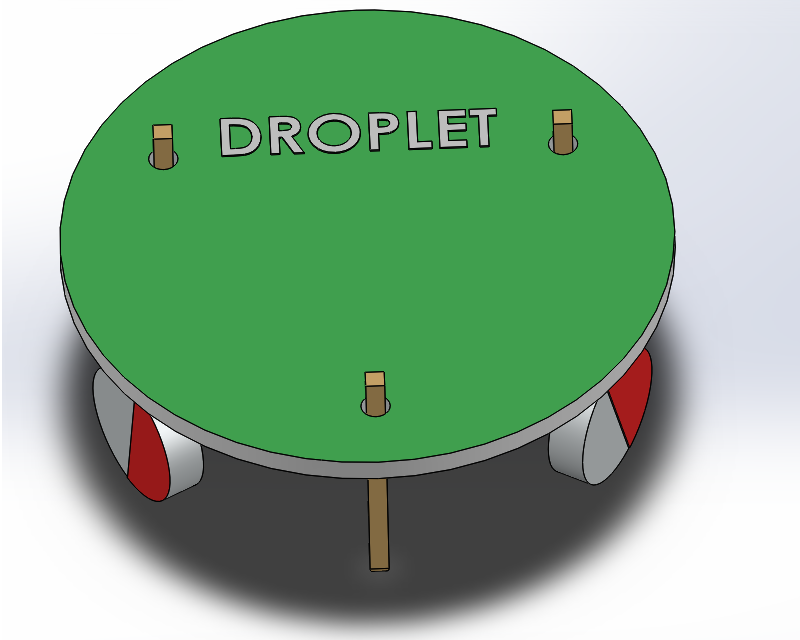
\includegraphics{Images/Walk.png}}{Images/Walk.swf}
			\end{figure}
			\note[item]<1->{This animation shows a robot walking by sequencing steps together.}
	\end{columns}
\end{frame}
\begin{frame}
	\frametitle{Calibration}
		\begin{itemize}
			\item Downside of low cost is inconsistent performance across different motors.
			\note[item]<1->{Now, one trade-off with these low-cost actuators is that the performance of the vibration motors varies.}
			\note[item]<1->{In order for the robot to walk straight, each individual step must be of the same magnitude. Without calibration, this is not the case.}
			\item To mitigate this problem, each robot is calibrated.
			\begin{itemize}
				\item If a motor tends to be weaker, turn it on for longer.
			\end{itemize}
			\note[item]<1->{Thus, we calibrate each robot by turning on weaker motors for slightly longer than other motors. In practice most of these adjustment values are around 3ms, or 10\% longer.}
			\item We also present a method for automatic calibration.
			\note[item]<1->{Details on the automatic calibration available during poster session.}
		\end{itemize}
\end{frame}
\end{document}